\documentclass[12pt,a4paper]{article}
\usepackage[utf8]{inputenc}
\usepackage[T1]{fontenc}
\usepackage{graphicx}
\usepackage{charter} % Font scelto per il documento
\usepackage{microtype}  % Migliora la qualità tipografica
\usepackage{titling}    % Per personalizzare il titolo
\usepackage[a4paper, margin=2cm]{geometry} % Imposta i margini
\usepackage{setspace} % Per gestire l'interlinea
\setstretch{1.1}  % interlinea di 1.1
\usepackage{enumitem}
\setlist{nolistsep} % Rimuove lo spazio tra gli elementi della lista
\usepackage{float} % Da inserire nel preambolo
\usepackage{wrapfig} % Pacchetto per posizionare testo e immagine affiancati
\usepackage{subfig} % Pacchetto per affiancare immagini
\renewcommand{\thefigure}{\arabic{figure}}
%\setcounter{figure}{6}
\usepackage[hidelinks]{hyperref}  % 'hidelinks' rimuove i bordi rossi
\usepackage{booktabs} % Per migliorare la qualità della tabella
\usepackage{array}    % Per una migliore gestione delle colonne
\usepackage{tabularx}
\usepackage{placeins}
\usepackage{pifont} % Pacchetto per i simboli
\usepackage{fontawesome} % Pacchetto per le icone FontAwesome
\usepackage[normalem]{ulem} % Pacchetto per sottolineature personalizzate
\usepackage{amssymb} % Pacchetto per simboli come \checkmark

\usepackage[most]{tcolorbox}
\usepackage{listings}
\usepackage{xcolor}
\usepackage[utf8]{inputenc}


% Rimuovi numeri di pagina sulla prima pagina
\thispagestyle{empty}

% Personalizza titolo (vuoto per ora, lo ricreeremo manualmente)
\title{}
\author{}
\date{}

\begin{document}

    % Creo la copertina manualmente
    \begin{titlepage}
        \begin{center}
            {\Large {UNIVERSITÀ DEGLI STUDI DI SASSARI}}

            \vspace*{\fill}

            {\large Progetto di fine corso:}

            \vspace{1cm}

            {\Large \textbf{PRESENTAZIONE DELLA BASE DATI "OwlBreak"}}
            \vspace{0.3cm}
            \begin{figure}[ht]
                \centering
                
\includegraphics[width=0.4\textwidth]{figures/logo.pdf}       
                \label{fig:logo} % Removed duplicate label to avoid error
            \end{figure}
     
            \vspace*{\fill}

            \begin{tabular}{l@{\hspace{2cm}}l}
                Studente: & Matricola: \\
                Daniele Picciau & 50056771 \\
                Monica Manai & 50057077
            \end{tabular}

            \vspace{2cm}

            {\large ANNO ACCADEMICO 2024-2025}
        \end{center}
    \end{titlepage}

    \section*{\hspace{15cm}Indice}
    \hrulefill 
    \renewcommand{\contentsname}{} % Rimuove completamente il titolo
    \tableofcontents
    \newpage

    % Introduzione
    \section{Analisi dei requisiti}
    \subsection{Descrizione del sistema informativo}
    \label{par:Descrizione del sistema informativo}
    Si vuole realizzare una base dati per la gestione del bar di una scuola secondaria (di primo o secondo grado) per il quale si vogliono rappresentare:
    \begin{itemize}[leftmargin=1em]
        \item I \textit{Clienti}, che siano essi studenti o personale scolastico, i quali possono effettuare \textit{Ordini} verso gli \textit{Operatori} del bar;
        \item Gli \textit{Ordini} effettuati dai \textit{Clienti};
        \item I \textit{Prodotti} disponibili per essere ordinati dai \textit{Clienti};
        \item Gli \textit{Ingredienti} necessari per la composizione di un \textit{Prodotto};
        \item Gli \textit{Operatori} del bar, i quali si occuperanno di gestire gli ordini dei \textit{Clienti} e di effetuare a loro volta delle richieste di \textit{Rifornimento};
        \item Le \textit{Assegnazioni}, che si occupano di associare un determinato luogo di consegna ad uno specifico \textit{Operatore};
        \item I \textit{Rifornimenti} richiesti dagli \textit{Operatori} per l'acquisto degli \textit{Ingredienti};
        \item I \textit{Fornitori} che possono visionare le richieste di \textit{Rifornimento} degli \textit{Operatori}.
    \end{itemize}

    \vspace{8pt}
    \noindent
    Per i \textit{Clienti}, identificati dall'email istituzionale, si vuole memorizzare il nome e il cognome e password. Nel caso in cui il cliente sia uno Studente, il sistema registrerà anche la classe di appartenenza. Se, invece, il cliente appartiene al Personale scolastico, verranno archiviati ulteriori dettagli, tra cui il ruolo ricoperto all'interno dell'istituto e il luogo di consegna predefinito degli ordini. Questa distinzione si rende necessaria poiché i membri del personale scolastico, non avendo una postazione fissa all'interno della scuola, devono poter specificare un punto di consegna per ricevere gli ordini in modo più efficiente.\\
    Inoltre, tra i ruoli del personale scolastico, gli unici utenti con privilegi amministrativi aggiuntivi sono gli "\textit{addetti alla segreteria}", che hanno la facoltà di creare, eliminare e modificare gli account dei clienti, siano essi studenti o membri del personale scolastico.

    \vspace{8pt}
    \noindent
    Gli \textit{Ordini} sono identificati dall'email istituzionale del cliente che ha effettuato l'ordine, dal nome del prodotto ordinato, dalla data e dall'ora in cui l'ordine è stato effettuato. Inoltre si vuole memorizzare l'avvenuta consegna dell'ordine da parte degli operatori.
    
    \vspace{8pt}
    \noindent
    Per i \textit{Prodotti}, identificati dal loro nome, si vuole memorizzare il prezzo e un indicatore di disponibilità. Quest'ultimo segnala se almeno uno degli ingredienti necessari alla preparazione del prodotto non è più disponibile, rendendolo temporaneamente non vendibile.

    \vspace{8pt}
    \noindent
    Per gli \textit{Ingredienti},  identificati dal loro nome, si vuole memorizzare una quantità, che indica il numero di unità disponibili, e l'elenco degli allergeni eventualmente contenuti.

    \vspace{8pt}
    \noindent
    Per gli \textit{Operatori}, identificati da un codice ID, si vuole memorizzare la propria email, la password, il nome, il cognome e il ruolo ricoperto all'interno del bar.\\
    Esistono diversi ruoli, ognuno con privilegi specifici, ma tutti gli operatori hanno la possibilità di visualizzare gli ordini effettuati dai clienti:
    \begin{itemize}[leftmargin=1em]
        \item Titolare: è l'unico operatore con la facoltà di aggiungere ed eliminare i dipendenti, oltre a disporre di tutti i permessi riservati agli altri ruoli;
        \item Addetti alle consegne: oltre al titolare, sono gli unici operatori autorizzati a confermare l'avvenuta consegna di un ordine;
        \item Addetti alle vendite: oltre al titolare, sono gli unici operatori abilitati a effettuare e visualizzare le richieste di rifornimento verso i fornitori, nonché a confermarne l'avvenuta consegna. Sono anche responsabili della vendita al bancone e della preparazione degli ordini.
    \end{itemize}

    \vspace{8pt}
    \noindent
    Le \textit{Assegnazioni} sono identificate da un luogo di consegna il cui obiettivo è quello di definire le aree di competenza degli \textit{"addetti alle consegne"} per la gestione degli ordini.

    \vspace{8pt}
    \noindent
    Per i \textit{Rifornimenti}, identificati da un codice ID, si vuole memorizzare l'ingrediente richiesto, la quantità ordinata, la data e l'ora dell'ordine, nonché l'avvenuta consegna da parte dei fornitori.

    \vspace{8pt}
    \noindent
    Per i \textit{Fornitori}, identificati da un codice ID, si vuole memorizzare il nome dell'azienda fornitrice, il nome del titolare, un indirizzo email di riferimento per eventuali comunicazioni o risoluzione di problematiche e la password.

    \subsection{Glossario dei termini}
    \begin{table}[h]
        \renewcommand{\arraystretch}{1.3} % Per aumentare la spaziatura tra le righe
        \centering
        \begin{tabular}{|m{3cm}|m{6cm}|m{3cm}|m{3cm}|}
            \hline
            \textbf{Termine} & \textbf{Descrizione} & \textbf{Sinonimi} & \textbf{Collegamenti} \\
            \hline
            Cliente & Utente con la sola possibilità di effettuare e visualizzare gli ordini. Può essere uno studente o un membro del personale scolastico. & Acquirente & Ordine \\
            \hline
            Ordine & Contiene le caratteristiche dell'ordine effettuato dal Cliente. & Richiesta & Prodotto, Operatore, Cliente \\
            \hline
            Prodotto & Indica un elemento disponibile o non per l'ordinazione. & Articolo & Ingrediente, Ordine \\
            \hline
            Ingrediente & Materia prima utilizzata per la preparazione dei Prodotti. & Componente & Prodotto \\
            \hline
            Operatore & Utente autorizzato alla gestione degli ordini e della vendita. Può effettuare richieste di rifornimento. & Addetto, Venditore & Ordine, Rifornimento \\
            \hline
            Assegnazione & Permette di definire le aree di competenza degli operatori per la distribuzione degli ordini & Incarico, Area assegnata & Operatore \\
            \hline
            Rifornimento & Richiesta di approvvigionamento di Ingredienti ai Fornitori. & Fornitura & Fornitore, Operatore \\
            \hline
            Fornitore & Utente responsabile della fornitura di Ingredienti al sistema, autorizzato alla visualizzazione delle richieste di rifornimento effettuate dagli operatori. & Azienda, Grossista & Rifornimento, Ingrediente \\
            \hline
        \end{tabular}
        \caption{Descrizione dei termini utilizzati nel sistema}
        \label{tab:termini}
        \vspace{-20pt}
    \end{table}

    \subsection{Elenco delle operazioni}
    \subsubsection{Operazioni di inserimento}
    \begin{enumerate}[leftmargin=2.8em,label=\textbf{Op.\arabic*}]
        \item Inserimento di un nuovo cliente nel sistema;
        \item Inserimento di un nuovo operatore nel sistema;
        \item Inserimento di una nuova richiesta di rifornimento da parte di un operatore verso un fornitore;
        \item Inserimento di un nuovo ordine da parte di un cliente (implica la rimozione della quantità corrispondente di ingredienti dal sistema).
        \item Inserimento di un nuovo fornitore nel sistema;
        \item Inserimento di un nuovo prodotto nel sistema;
        \item Inserimento di un nuovo ingrediente nel sistema;
    \end{enumerate}

    \subsubsection{Operazioni di modifica}
    \begin{enumerate}[leftmargin=2.8em,label=\textbf{Op.\arabic*}]
        \item Modifica dei dati di un cliente;
        \item Modifica dei dati di un operatore;
        \item Modifica dei dati di un fornitore;
    \end{enumerate}

    \subsubsection{Operazioni di eliminazione}
    \begin{enumerate}[leftmargin=2.8em,label=\textbf{Op.\arabic*}]
        \item Eliminazione di un cliente dal sistema;
        \item Eliminazione di un operatore dal sistema;
        \item Eliminazione di un fornitore dal sistema;
    \end{enumerate}

    \subsubsection{Operazioni di conferma e aggiornamento}
    \begin{enumerate}[leftmargin=2.8em,label=\textbf{Op.\arabic*}]
        \item Conferma della consegna di un ordine da parte di un operatore;
        \item Conferma della consegna di un rifornimento da parte di un fornitore (implica l'aggiornamento delle scorte di ingredienti, con eventuale inserimento di nuovi ingredienti se necessario).
        \item Aggiornamento della quantità di un ingrediente dopo un ordine;
        \item Aggiornamento della quantità di un ingrediente dopo un rifornimento;
        \item Aggiornamento della disponibilità di un prodotto;
    \end{enumerate}

    \subsubsection{Operazioni di visualizzazione}
    \begin{enumerate}[leftmargin=2.8em,label=\textbf{Op.\arabic*}]
        \item Visualizzazione degli ordini giornalieri di un singolo cliente;
        \item Visualizzazione della cronologia ordini di un singolo cliente;
        \item Visualizzazione del prezzo totale di un ordine da parte di un cliente;
        \item Visualizzazione dei prodotti disponibili ad essere ordinati.
        \item Visualizzazione, per gli operatori, degli ordini giornalieri suddivisi per luogo di consegna;
        \item Visualizzazione dei dati relativi ai fornitori da parte degli operatori;
        \item Visualizzazione delle richieste di rifornimento da parte degli operatori, raggruppate per fornitore;
        \item Visualizzazione delle richieste di rifornimento da parte dei fornitori, limitata alle richieste a loro indirizzate.
    \end{enumerate}

    \newpage
    \section{Modellazione concettuale} 
    La modellazione concettuale rappresenta un passaggio fondamentale nella progettazione del sistema, in quanto consente di definire in modo chiaro e strutturato le entità coinvolte e le relazioni tra di esse.\\
    Attraverso l'uso del modello Entità-Relazione (E-R), è possibile ottenere una rappresentazione visiva e formale della logica del database, facilitando l'analisi e la comprensione del dominio applicativo. In questa parte verrà illustrato lo schema E-R del sistema, mettendo in evidenza le principali entità e relazioni. Successivamente, verranno descritte le cardinalità e i vincoli che regolano il funzionamento del sistema in esame.

    \subsection{Schema E-R}
    \begin{figure}[H]
        \centering
        \vspace{-20pt}  % Riduce lo spazio sopra
        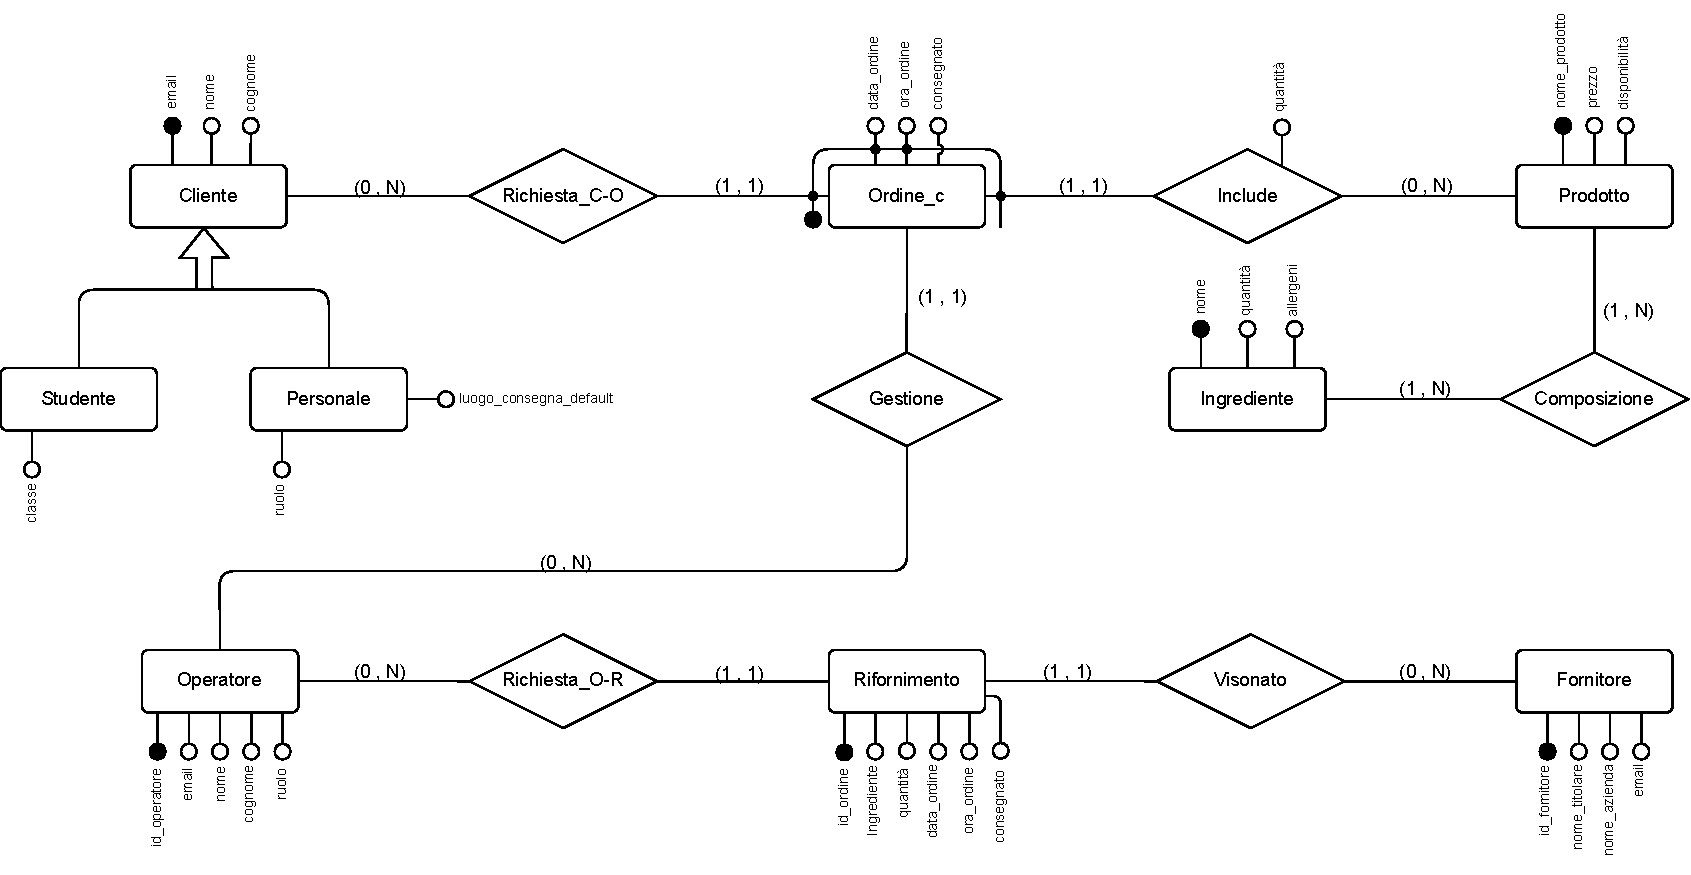
\includegraphics[width=1\textwidth]{figures/Conceptual_model.pdf}
        \vspace{-20pt}  % Riduce lo spazio sopra
        \caption{Modello entità-relazione}
        \label{fig:Conceptual_model}
    \end{figure} 

    \subsection{Descrizione dei vincoli}
    \subsubsection{Cardinalità}
    \begin{itemize}[leftmargin=1em]
        \item \textbf{Richiesta\_C-O} (1:\(N\)): Un cliente può effettuare da 0 a \(N\) ordini, mentre un ordine è effettuato da uno e un solo cliente;
        \item \textbf{Include} (1:\(N\)): Un ordine include uno e un solo prodotto, mentre un prodotto può essere incluso in 0 o \(N\) ordini;
        \item \textbf{Composizione} (\(N\):\(N\)): Un prodotto è composto da 1 o \(N\) ingredienti, mentre un ingrediente può essere parte di 1 o \(N\) prodotti;
        \item \textbf{Gestione} (1:\(N\)): Un ordine è gestito da uno e un solo operatore, mentre un operatore può gestire da 0 a \(N\) ordini;
        \item \textbf{Associamento} (1:\(N\)): Un operatore può essere associato da 0 a \(N\) assegnazioni, mentre un'assegnazione è associata ad uno e un solo operatore;
        \item \textbf{Richiesta\_O-R} (1:\(N\)): Un operatore può effettuare da 0 a \(N\) richieste di rifornimento, mentre una richiesta di rifornimento è effettuata da uno e un solo operatore;
        \item \textbf{Visionato} (1:\(N\)): Un fornitore può visionare da 0 a \(N\) richieste di rifornimento, mentre una richiesta di rifornimento è visionata da uno e un solo fornitore;
    \end{itemize}

    \subsubsection{Regole di vincolo non esprimibili nello schema}
    \begin{enumerate}[leftmargin=3em,label=\textbf{(RV\arabic*)}]
        \item  Gli ordini devono essere effettuati tra le 8 e le 10 del mattino;
        \item La quantità di ogni ingrediente deve essere aggiornata ogni volta che viene effettuato un ordine;
        \item La quantità di ogni ingrediente deve essere aggiornata ogni volta che un rifornimento viene consegnato;
        \item La disponibilità dei prodotti deve essere aggiornata dopo ogni aggiornamento ed eliminazione di un ingrediente;
        \item La disponibilità dei prodotti deve essere aggiornata dopo ogni inderimento ed eliminazione di una composizione;
        \item Un cliente può modificare il proprio luogo consegan solo se il suo tipo non è "\textit{Studente}";
        \item Un nuovo cliente può essere aggiunto solo da clienti con tipo "\textit{Addetto-Segreteria}";
        \item Un nuovo operatore può essere aggiunto solo da clienti con tipo "\textit{Titolare}";
        \item Un ordine può essere consegnato solo da un operatore con tipo "\textit{Addetto-Consegna}";
        \item Un rifornimento può essere richiesto solo da un operatore con tipo "\textit{Addetto-Vendite}" o "\textit{Titolare}";
        \item Un rifornimento può essere segnato come consegnato solo da un operatore con tipo "\textit{Addetto-Vendite}" o "\textit{Titolare}";
    \end{enumerate}

    \subsubsection{Regole di derivazione}
    \begin{enumerate}[leftmargin=3em,label=\textbf{(RD\arabic*)}]
        \item  Il numero di ordini effettuati da un cliente può essere calcolato contando le istanze della relazione Richiesta\_C-O associate a quel cliente.
        \item Il numero di ordini effettuati da un cliente si orriene calcolando il numero di tuple dove la mail del cliente coincide con l'email del cliente che ha effettuato l'ordine;
        \item Il totale speso in ordini da un determinato cliente può essere calcolato sommando i prezzi dei prodotti inclusi negli ordini effettuati da quel cliente.
        \item La media spesa per ordine di un determinato cliente può essere calcolata dividendo il totale speso in ordini per il numero di ordini effettuati da quel cliente.
        \item Gli ordini associati ad un determinato operatore "\textit{Addetto-Consegna}" possono essere ottenuti grazie ai luoghi di consegna associati a quell'operatore nella tabella Assegnazione, e filtrando gli ordini in base al luogo di consegana associato al cliente che ha effettuato l'ordine; 
    \end{enumerate}

    \newpage
    \section{Modellazione logica}
    Dopo aver definito la struttura del modello relazionale, è possibile analizzare le operazioni  di ristrutturazione dello schema E-R in vista della successiva normalizzazione. Verranno illustrate varie tecniche, tra cui l'eliminazione delle generalizzazioni presenti nel modello concettuale.

    \subsection{Ristrutturazione dello schema E-R}
    \subsubsection{Eliminazione delle generalizzazioni}
    All'interno della base dati in esame è presente una generalizzazione totale, perché ogni istanza dell'entità generale \textit{Cliente} appartiene obbligatoriamente a una sotto-entità \textit{Studente} e \textit{Personale}. Non ci sono quindi clienti che non siano studenti o membri del personale scolastico.\\
    Inoltre la generalizzazione è esclusiva perché ogni istanza di \textit{Cliente} appartiene a una sola sotto-entità, un cliente non può essere contemporaneamente uno studente e un membro del personale scolastico.

    \vspace{8pt}
    \noindent
    I sistemi tradizionali per la gestione della base dati non consentono la rappresentazione delle generalizzazioni, ragion per cui, risulta necessario trasformarle in costrutti per i quali esiste un implementazione naturale, come entità e associazioni.\\
    Per risolvere questo tipo di generaizzazione è stato scelto di utilizzare un \textbf{accorpamento delle entità figlie della generalizzazione nell'entità genitore}: in questo caso le entità \textit{Studente} e \textit{Personale} sono state eliminate e le loro proprietà vengono aggiunte all'entità \textit{Cliente} con qualche accorgimento.
    
    \vspace{8pt}
    \noindent
    In paricolare, l'attributo \textbf{classe} e l'attributo \textbf{ruolo} vengono eliminati e sostituiti dall'attributo \textbf{tipoCliente}. Per fare in modo di rimanere coerenti con la descrizione iniziale del sistema, il \textbf{tipoCliente} può assumere i seguenti valori.\\
    Se il \textbf{tipoCliente} è "\textit{Studente}", il cliente in questione non ha la possibilità di modificare il valore dell'attributo \textbf{luogoConsegna} che coinciderà con la propria classe di appartenenza.
    Al contrario il cliente in questione avrà la facoltà di modificare il valore dell'attributo \textbf{luogoConsegna}, inoltre se l'attributo \textbf{tipoCliente} coincide con "\textit{addetto alla segreteria}", quest'utlimo avrà in più i privilegi descritti al paragrafo~\ref{par:Descrizione del sistema informativo}.\\
    \begin{figure}[H]
        \centering
        \vspace{-20pt}  % Riduce lo spazio sopra
        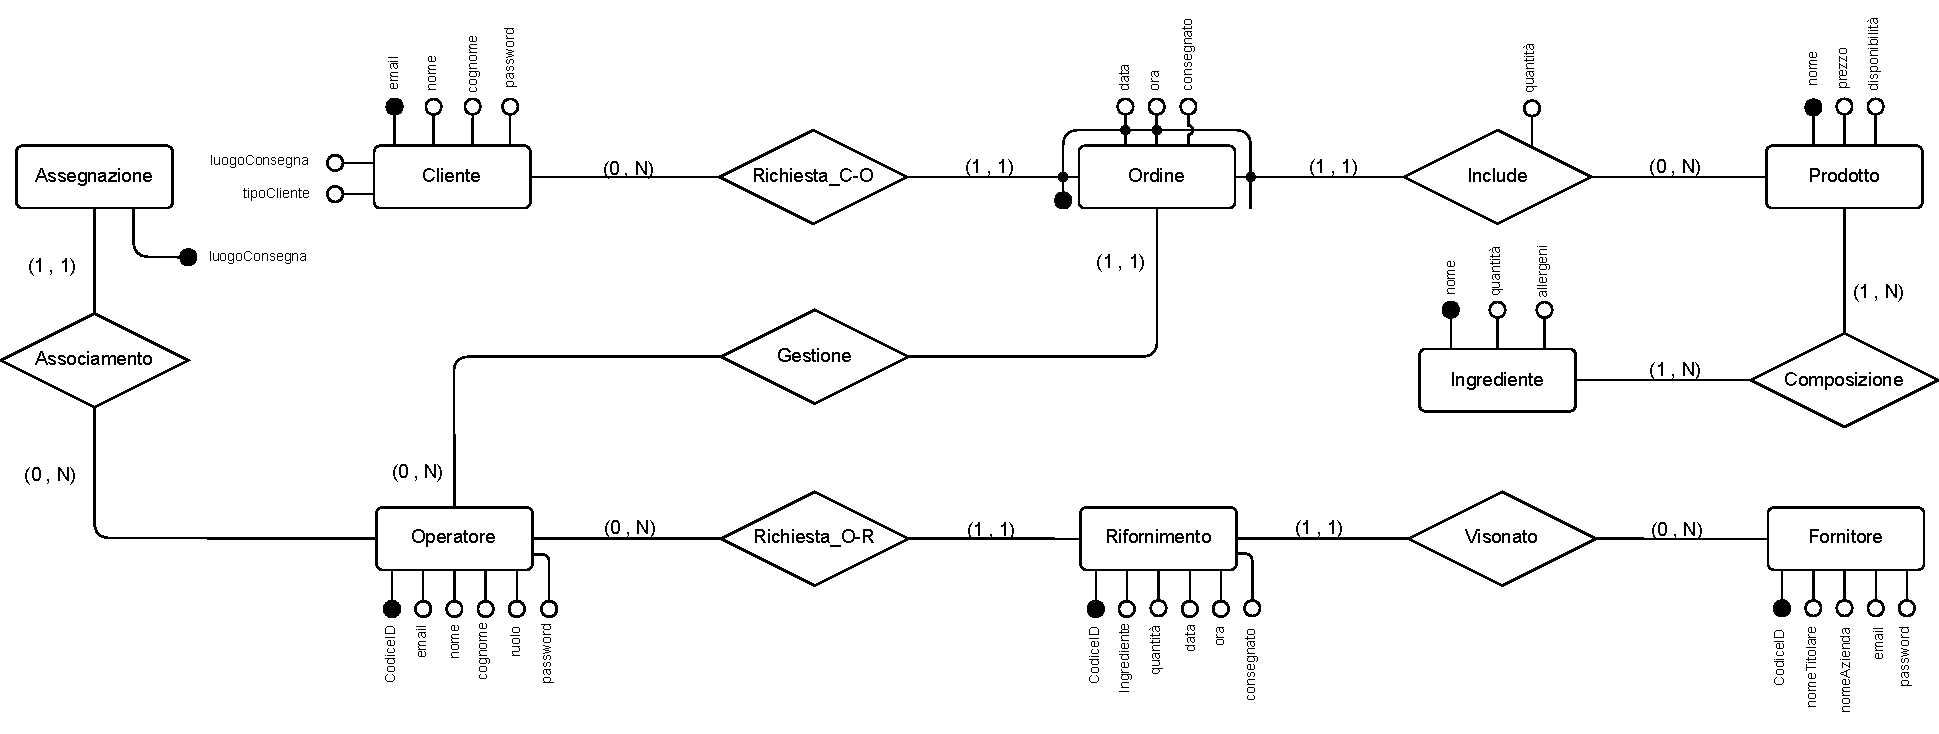
\includegraphics[width=\textwidth]{figures/Conceptual_model2.pdf}
        \vspace{-20pt}  % Riduce lo spazio sopra
        \caption{Modello entità-relazione ristrutturato}
        \label{fig:Conceptual_model2}
    \end{figure} 
    

    \subsection{Tavola dei volumi}
    \begin{table}[ht]
        \captionsetup{justification=raggedright, singlelinecheck=false}
        \renewcommand{\arraystretch}{1.3} % Per aumentare la s
        \begin{tabular}{| >{\centering\arraybackslash}m{3cm}| >{\centering\arraybackslash}m{2cm}| >{\centering\arraybackslash}m{3cm}|}
            \hline
            \textbf{Concetto} & \textbf{Tipo} & \textbf{Volume}\\
            \hline
            Cliente & E & 700 \\
            \hline
            Ordine & E  & 1400\\
            \hline
            Prodotto & E & 120\\
            \hline
            Ingrediente & E & 35\\
            \hline
            Operatore & E & 10\\
            \hline
            Assegnazione & E & 30\\
            \hline
            Rifornimento & E & 35\\
            \hline
            Fornitore & E & 6\\
            \hline
            Richiesta\_C-O & R & 1400\\
            \hline
            Include & R & 1400\\
            \hline
            Composizione & R & 95\\
            \hline
            Gestione & R & 1400\\
            \hline
            Associamento & R & 30\\
            \hline
            Richiesta\_O-R & R & 35\\ 
            \hline
            Visionato & R & 35\\ 
            \hline     
        \end{tabular}
        \caption{Concetti dello schema con i volumi previsti a regime}
        \label{tab:tavola_volumi}
        \vspace{-21pt}
    \end{table}

    \subsubsection{Volume delle associazioni}
    \noindent
    Nella tavola dei volumi il numero delle occorrenze delle associazioni (R) dipende da due parametri:
    \begin{enumerate}[leftmargin=1.3em]
        \item \textbf{Parametro delle occorrenze delle entità}: il primo parametro dipende dal numero di occorrenze delle entità coinvolte nelle associazioni e dal numero (medio) di partecipazioni di un'occorrenza di entità alle occorrenze di associazioni;
        \item \textbf{Parametro delle cardinalità}: il secondo parametro dipende a sua volta dalle cardinalità delle associazioni.
    \end{enumerate}

    \vspace{8pt}
    \noindent
    Avendo una stima del numero di occorrenze delle entità, è possibile calcolare il numero di occorrenze delle associazioni:
    \begin{itemize}[leftmargin=1em]
        \item \textbf{Composizione}: Non tutti gli ingredienti vengono utilizzati nella composizione di un prodotto, poiché alcuni ingredienti possono essere forniti già pronti per la vendita, senza necessità di preparazione. Per questo motivo, si stima che il numero di occorrenze della relazione \textit{Composizione} sia pari a 95;
        \item  \textbf{Richiesta\_C-O}: il numero di occorrenze è pari al numero di \textit{Ordini}, poiché dalla cardinalità si evince che un ordine è richiesto da un solo cliente;
        \item \textbf{Include}: il numero di occorrenze è pari al numero degli \textit{Ordini}, in quanto ogni tupla di ogni  di \textit{Ordini} include un solo prodotto;
        \item \textbf{Gestione}: il numero di occorrenze è pari a quello degli \textit{Ordini}, poiché ogni ordine viene gestito singolarmente da un operatore;
        \item \textbf{Associamento}: il numero di occorrenze è pari al numero di \textit{Assegnazioni}, poiché dalla cardinalità si evince che ogni assegnazione è associata ad un solo operatore; 
        \item \textbf{Richiesta\_O-R}: il numero di occorrenze coincide con il numero dei \textit{Rifornimenti}, poiché dalla
        cardinalità si evince che  ogni rifornimento è richiesto da un solo operatore;
        \item \textbf{Visionato}: Anche in questo caso, il numero delle occorrenze è pari al numero dei \textit{Rifornimenti},  perché ogni rifornimento è visionato da un solo fornitore.
    \end{itemize}



    \subsection{Tavole delle operazioni}
    \begin{table}[ht]
        \centering
        \renewcommand{\arraystretch}{1.3}

        \begin{tabular}{| >{\centering\arraybackslash}m{2.5cm}| >{\centering\arraybackslash}m{1cm}| >{\centering\arraybackslash}m{3.5cm}|}
            \hline
            \textbf{Operazione} & \textbf{Tipo} & \textbf{Frequenza} \\
            \hline
            Op. 1  & I & 1400 al giorno\\
            \hline
            Op. 2 & I & 700 a settimana\\
            \hline
            Op. 3 & I & 700 al giorno\\
            \hline
            Op. 4 & I & 700 al giorno\\
            \hline
            Op. 5 & I & 10 al giorno\\
            \hline
            Op. 6 & I & 1 ogni 2 settimane\\
            \hline
            Op. 7 & I & 1 al giorno\\
            \hline
            Op. 8 & I & 1 al giorno\\
            \hline
        \end{tabular}
        \caption*{\textbf{Operazioni di visualizzazione}}

        \vspace{0.5cm}

        \begin{minipage}{0.45\textwidth}
            \centering
            \begin{tabular}{|>{\centering\arraybackslash}m{2.5cm}|>{\centering\arraybackslash}m{1cm}|>{\centering\arraybackslash}m{3cm}|}
                \hline
                \textbf{Operazione} & \textbf{Tipo} & \textbf{Frequenza} \\
                \hline
                Op. 1 & I & 125 all'anno \\
                \hline
                Op. 2 & I & 3 all'anno\\
                \hline
                Op. 3 & I & 35 al giorno\\
                \hline
                Op. 4 & I & 1400 al giorno\\
                \hline
                Op. 5 & I & 3 all'anno\\
                \hline
                Op.6 & I & 7 all'anno\\
                \hline
                Op.7 & I & 14 all'anno \\
                \hline
            \end{tabular}
            \caption*{\textbf{Operazioni di inserimento}}
        \end{minipage}
        \hspace{1cm}
        \begin{minipage}{0.45\textwidth}
            \centering
            \begin{tabular}{|>{\centering\arraybackslash}m{2.5cm}|>{\centering\arraybackslash}m{1cm}|>{\centering\arraybackslash}m{3cm}|}
                \hline
                \textbf{Operazione} & \textbf{Tipo} & \textbf{Frequenza} \\
                \hline
                Op. 1 & I & 1400 al giorno\\
                \hline
                Op. 2 & I & 35 al giorno\\
                \hline
                Op.3 & I & 1400 al giorno\\
                \hline
                Op.4 & I & 35 al giorno\\
                \hline
                Op.5 & I & 1435 al giorno\\
                \hline
            \end{tabular}
            \begin{center}
                \textbf{Operazioni di conferma e aggiornamento}
            \end{center}
        \end{minipage}
    \end{table}
    \vspace{-0.5cm}
    \begin{table}[ht]
        \centering
        \renewcommand{\arraystretch}{1.3}
        \begin{minipage}{0.45\textwidth}
            \centering
            \begin{tabular}{|>{\centering\arraybackslash}m{2.5cm}|>{\centering\arraybackslash}m{1cm}|>{\centering\arraybackslash}m{3cm}|}
                \hline
                \textbf{Operazione} & \textbf{Tipo} & \textbf{Frequenza} \\
                \hline
                Op. 1 & I & 500 all'anno\\
                \hline
                Op. 2 & I & 3 all'anno\\
                \hline
                Op. 3 & I & 2 a settimana\\
                \hline
            \end{tabular}
            \caption*{\textbf{Operazioni di modifica}}
        \end{minipage}
        \hspace{1cm}
        \begin{minipage}{0.45\textwidth}
            \centering
            \begin{tabular}{|>{\centering\arraybackslash}m{2.5cm}|>{\centering\arraybackslash}m{1cm}|>{\centering\arraybackslash}m{3cm}|}
                \hline
                \textbf{Operazione} & \textbf{Tipo} & \textbf{Frequenza}\\
                \hline
                Op. 1 & I & 125 all'anno\\
                \hline
                Op. 2 & I & 3 all'anno\\
                \hline
                Op. 3 & I & 3 all'anno\\
                \hline
            \end{tabular}
            \caption*{\textbf{Operazioni di cancellazione}}
        \end{minipage}
        \vspace{-4pt}
        \caption{Riepilogo delle operazioni previste nello schema}
        \label{tab:operazioni_4x}
    \end{table}
    
    \FloatBarrier
    \vspace{-8pt}
    \begin{tcolorbox}[
        colback=yellow!10, 
        colframe=yellow!50!black, 
        title=\faExclamationTriangle \quad Nota 
    ]
        Le frequenze indicate per le operazioni interattive (I) rappresentano stime medie del carico di lavoro previsto e possono variare in base all'utilizzo effettivo del sistema. Questi valori sono utilizzati come riferimento per il dimensionamento delle risorse e la valutazione delle prestazioni, ma non costituiscono limiti operativi.
    \end{tcolorbox}
    
    \subsection{Traduzione nel modello relazionale}
    \begin{tcolorbox}[
        colback=gray!8,
        colframe=black!30,
        title=
    ]
        \textbf{Cliente}(\textbf{\uline{email}}, password, nome, cognome, luogoConsegna, tipoCliente)
    \end{tcolorbox}

    \begin{tcolorbox}[
        colback=gray!8,
        colframe=black!30,
        title=
    ]
        \textbf{Ordine}(\uline{\textbf{data}}, \textbf{\uline{ora}}, \textbf{\uline{emailCliente}}, \textbf{\uline{nomeProdotto}}, consegnato, quantità, OperatoreID)
        \begin{itemize}[leftmargin=1em]
            \item \textit{OperatoreID} è chiave esterna di \textbf{Operatore}(CodiceID)
            \item \textit{emailCliente} è chiave esterna di \textbf{Cliente}(email) e allo stesso tempo appartiene alla chiave primaria
            \item \textit{nomeProdotto} è chiave esterna di \textbf{Prodotto}(nome) e allo stesso tempo appartiene alla chiave primaria
        \end{itemize}
    \end{tcolorbox}
    
    \begin{tcolorbox}[
        colback=gray!8,
        colframe=black!30,
        title=
    ]
        \textbf{Prodotto}(\textbf{\uline{nome}}, prezzo, disponibilità)
    \end{tcolorbox}

    \begin{tcolorbox}[
        colback=gray!8,
        colframe=black!30,
        title=
    ]
        \textbf{Composizione}(\textbf{\uline{nomeProdotto}}, \textbf{\uline{nomeIngrediente}})
        \begin{itemize}[leftmargin=1em]
            \item \textit{nomeProdotto} è chiave esterna di \textbf{Prodotto}(nome) e allo stesso tempo appartiene alla chiave primaria
            \item \textit{nomeIngrediente} è chiave esterna di \textbf{Ingrediente}(nome) e allo stesso tempo appartiene alla chiave primaria
        \end{itemize}
    \end{tcolorbox}

    \begin{tcolorbox}[
        colback=gray!8,
        colframe=black!30,
        title=
    ]
        \textbf{Ingrediente}(\textbf{\uline{nome}}, allergeni, quantità)
    \end{tcolorbox}

    \begin{tcolorbox}[
        colback=gray!8,
        colframe=black!30,
        title=
    ]
        \textbf{Operatore}(\textbf{\uline{CodiceID}}, email, password, nome, cognome, ruolo)
    \end{tcolorbox}

    \begin{tcolorbox}[
        colback=gray!8,
        colframe=black!30,
        title=
    ]
        \textbf{Assegnazione}(\textbf{\uline{LuogoConsegna}}, OperatoreID)
        \begin{itemize}[leftmargin=1em]
            \item \textit{OperatoreID} è chiave esterna di \textbf{Operatore}(CodiceID)
        \end{itemize}
    \end{tcolorbox}

    \begin{tcolorbox}[
        colback=gray!8,
        colframe=black!30,
        title=
    ]
        \textbf{Rifornimento}(\textbf{\uline{CodiceID}}, ingrediente, quantità, data, ora, consegnato, OperatoreID, \\FornitoreID)
        \begin{itemize}[leftmargin=1em]
            \item \textit{OperatoreID} è chiave esterna di \textbf{Operatore}(CodiceID)
            \item \textit{FornitoreID} è chiave esterna di \textbf{Fornitore}(CodiceID)
        \end{itemize}
    \end{tcolorbox}

    \begin{tcolorbox}[
        colback=gray!8,
        colframe=black!30,
        title=
    ]
        \textbf{Fornitore}(\textbf{\uline{CodiceID}}, nomeTitolare, nomeAzienda, email, password) 
    \end{tcolorbox}
    
    \subsubsection{Vincoli di integrità referenziale}
    \begin{itemize}[leftmargin=1em]
        \item FOREIGN KEY \textbf{Ordine}(emailCliente) REFERENCES \textbf{Cliente}(email)
        \item FOREIGN KEY \textbf{Ordine}(nomeProdotto) REFERENCES \textbf{Prodotto}(nome)
        \item FOREIGN KEY \textbf{Ordine}(OperatoreID) REFERENCES \textbf{Operatore}(CodiceID)
        \item FOREIGN KEY \textbf{Composizione}(nomeProdotto) REFERENCES \textbf{Prodotto}(nome)
        \item FOREIGN KEY \textbf{Composizione}(nomeIngrediente) REFERENCES \textbf{Ingrediente}(nome)
        \item FOREIGN KEY \textbf{Assegnazione}(OperatoreID) REFERENCES \textbf{Operatore}(CodiceID)
        \item FOREIGN KEY \textbf{Rifornimento}(OperatoreID) REFERENCES \textbf{Operatore}(CodiceID)
        \item FOREIGN KEY \textbf{Rifornimento}(FornitoreID) REFERENCES \textbf{Fornitore}(CodiceID)
    \end{itemize}

    \subsubsection{Modello relazionale}
    \begin{tcolorbox}[
        colback=gray!8,  
        colframe=darkgray, 
        title=Legenda del modello relazionale
    ]
        \begin{tabular}{@{} >{\centering\arraybackslash}m{0.5cm} p{14cm} @{}}
            
\includegraphics[width=0.025\textwidth]{figures/g132.pdf} & \textbf{Chiave primaria} (identificatore univoco della tabella) \\
            \addlinespace[0.5em]
            
\includegraphics[width=0.025\textwidth]{figures/path621.pdf} & \textbf{Chiave esterna} (collegamento a una chiave primaria di un'altra tabella) \\ 
        \end{tabular}
    \end{tcolorbox}  
     
    \begin{figure}[H]
        \centering 
        \vspace{-10pt}  % Riduce lo spazio sopra
        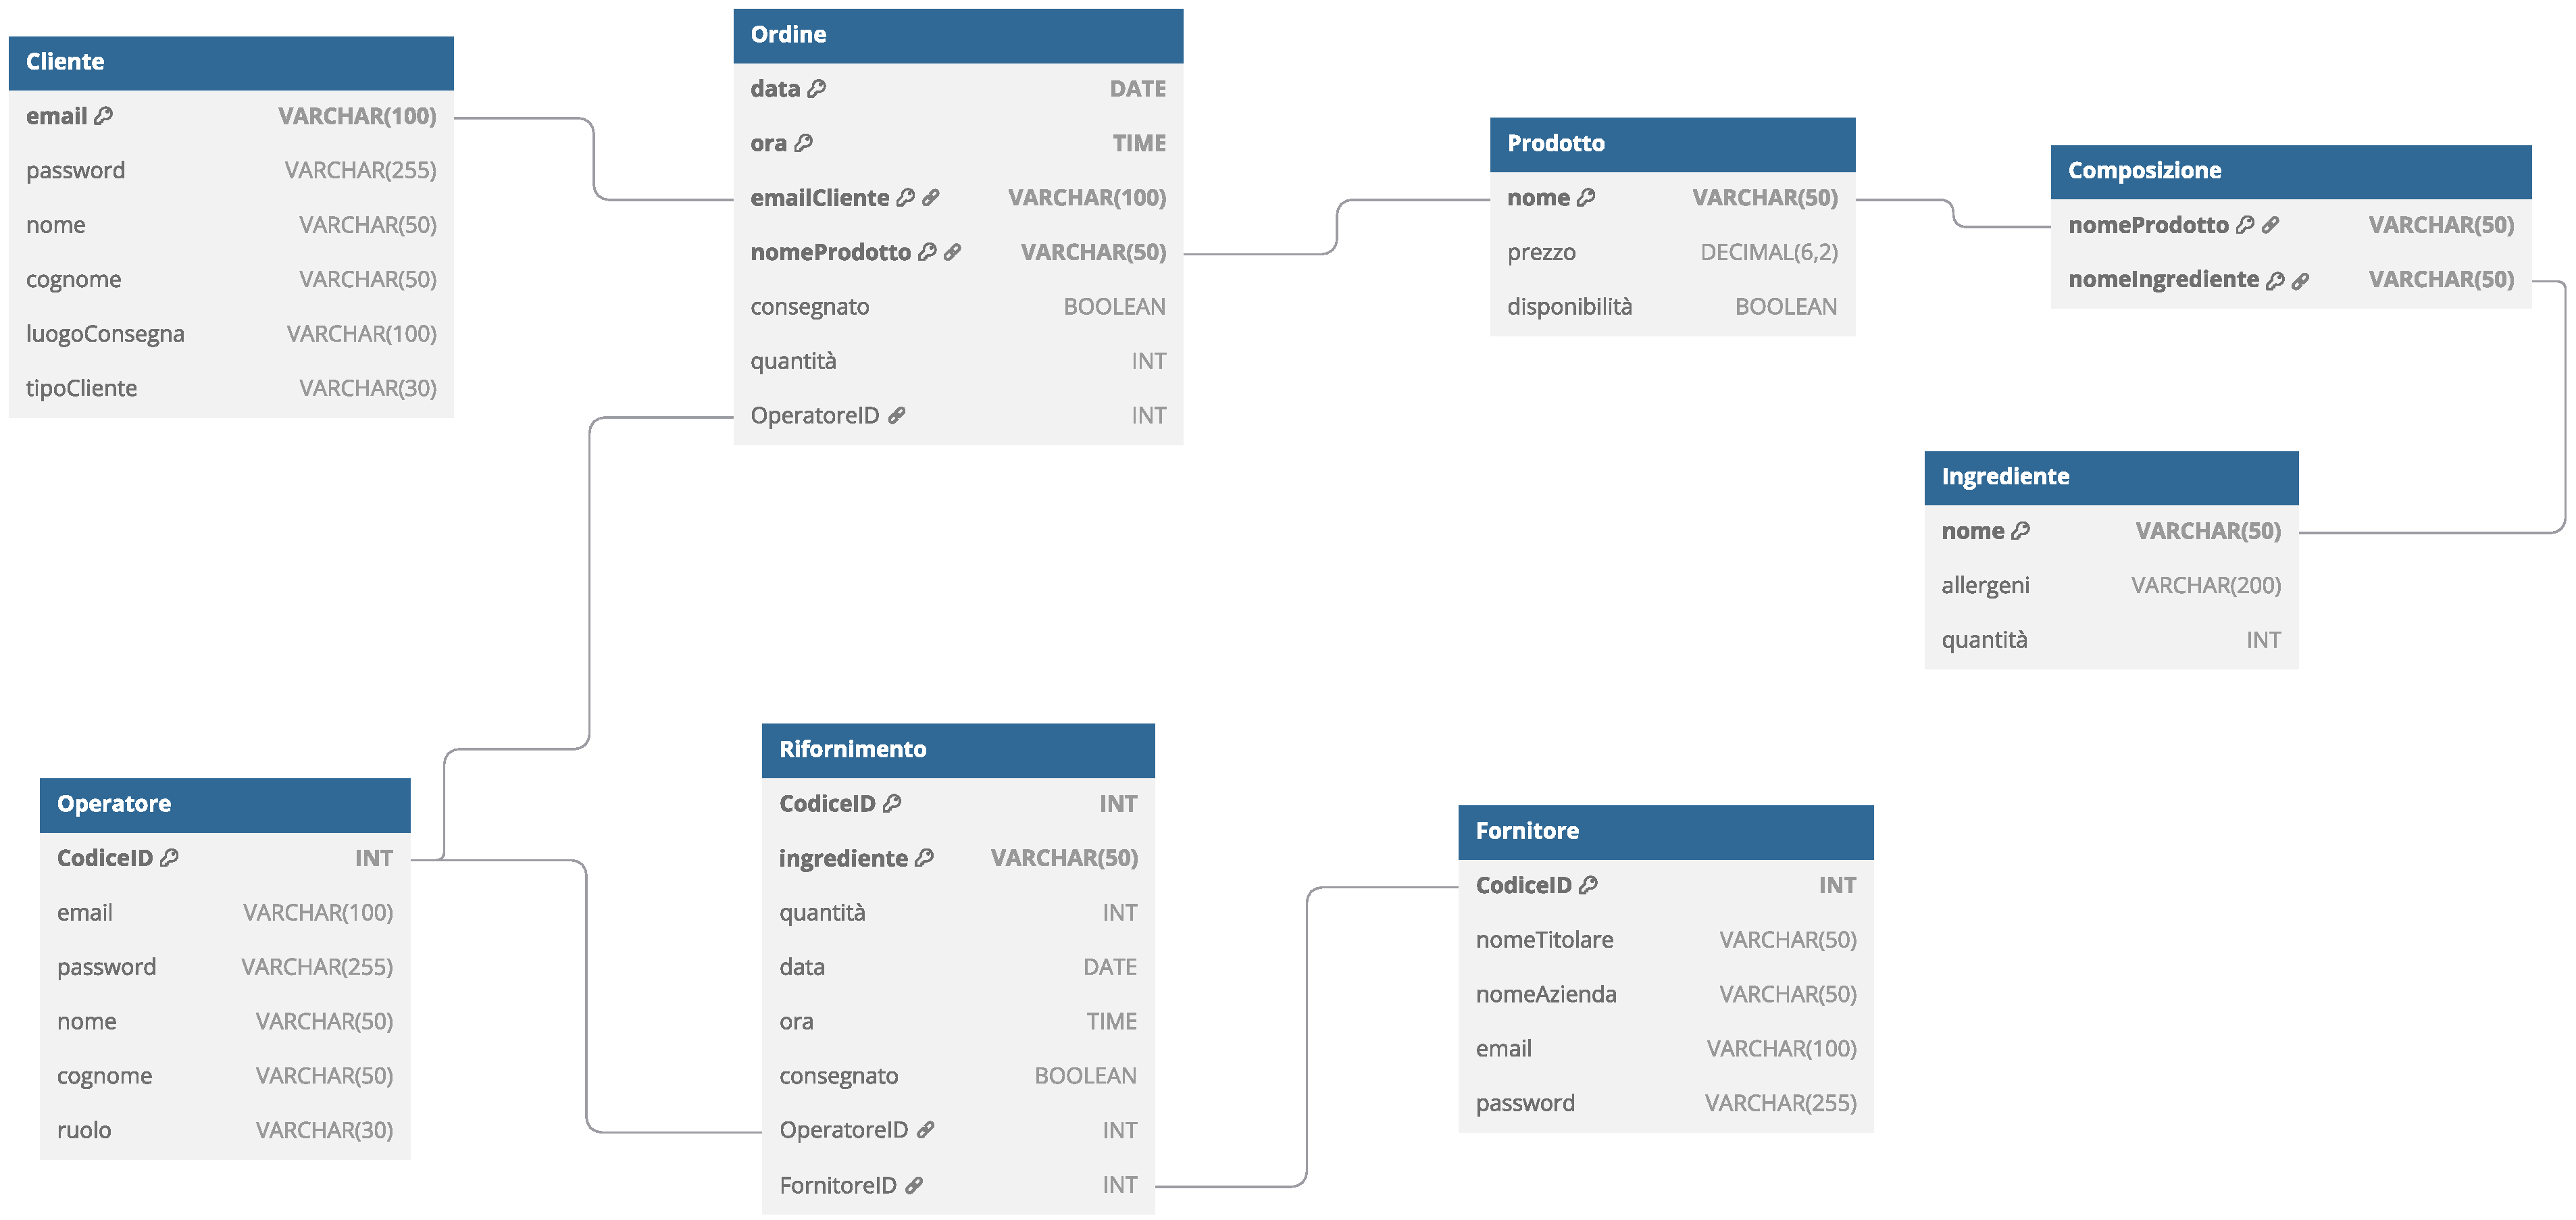
\includegraphics[width=\textwidth]{figures/Relational_model.pdf}
        \vspace{-20pt}  % Riduce lo spazio sopra
        \caption{Modello relazionale (collegamenti tra chiavi)}
    \end{figure}  

    \newpage
    \section{Normalizzazione}
    In questa sezione si procederà direttamente all'analisi della Terza Forma Normale (3NF), in quanto il rispetto di tale forma implica automaticamente il soddisfacimento dei requisiti previsti dalla Prima e dalla Seconda Forma Normale. \\
    Saranno quindi analizzate tutte le tabelle del modello relazionale, evidenziando per ciascuna le motivazioni per cui soddisfano i vincoli imposti dalla 3NF, con particolare attenzione alle dipendenze funzionali e alla struttura delle chiavi.

    \subsection{Tecniche di normalizzazione}
    Al fine di procedere con l'analisi, è opportuno fornire una definizione formale dei vincoli che caratterizzano la Terza Forma Normale (3NF).\\
    Affinché una relazione \textit{r} sia in 3NF, devono essere soddisfatte le seguenti condizioni:

    \begin{enumerate}[leftmargin=1.3em]
        \item Deve essere in 2NF, ovvero non deve presentare dipendenze funzionali parziali;
        \item Per ogni dipendenza funzionale \textit{X} $\rightarrow$ \textit{A}, deve essere verificata almeno una delle seguenti condizioni:
            \begin{enumerate}[leftmargin=1.3em, label=\alph*.]
            \item \textit{X} è una superchiave per \textit{r};
            \item \textit{A} appartiene ad almeno una chiave candidata di \textit{r}.
        \end{enumerate}
    \end{enumerate}

    \vspace{5pt}
    \noindent
    Infine, una relazione risulta essere anche in forma normale di Boyce-Codd (BCNF) qualora sia in 3NF e non presenti alcun tipo di dipendenza transitiva, incluse quelle ammesse dal punto \textit{2b} della 3NF.

    \subsubsection*{Tabella Cliente}
    \begin{tcolorbox}[
        colback=gray!8,
        colframe=black!30,
        title=
    ]
        \textbf{Cliente}(\textbf{\uline{email}}, password, nome, cognome, luogoConsegna, tipoCliente)
    \end{tcolorbox}

    \noindent
    La relazione \textit{Cliente} soddisfa i requisiti ai punti \textit{1} e \textit{2a}, quindi è in \textbf{3NF} e, non avendo dipendenze transitive come quelle riportate al punto \textit{2b}, è anche in \textbf{BCNF}.\\
    Di seguito vengono riportate le dipendenze funzionali della relazione \textit{Cliente}:
    \begin{itemize}[leftmargin=1em, label=$\circ$]
        \item email $\rightarrow$ password
        \item email $\rightarrow$ nome
        \item email $\rightarrow$ cognome
        \item email $\rightarrow$ luogoConsegna
        \item email $\rightarrow$ tipoCliente
    \end{itemize}
    
    \subsubsection*{Tabella Ordine}
    \begin{tcolorbox}[
        colback=gray!8,
        colframe=black!30,
        title=
    ]
        \textbf{Ordine}(\uline{\textbf{data}}, \textbf{\uline{ora}}, \textbf{\uline{emailCliente}}, \textbf{\uline{nomeProdotto}}, consegnato, quantità, OperatoreID)
    \end{tcolorbox}
    
    \noindent
    La relazione \textit{Ordine} soddisfa i requisiti ai punti \textit{1} e \textit{2a}, quindi è in \textbf{3NF} e, non avendo dipendenze transitive come quelle riportate al punto \textit{2b}, è anche in \textbf{BCNF}.\\
    Di seguito vengono riportate le dipendenze funzionali della relazione \textit{Ordine}:
    \begin{itemize}[leftmargin=1em, label=$\circ$]
        \item (data, ora, emailCliente, nomeProdotto) $\rightarrow$ consegnato
        \item (data, ora, emailCliente, nomeProdotto) $\rightarrow$ quantità
        \item (data, ora, emailCliente, nomeProdotto) $\rightarrow$ OperatoreID
    
    \end{itemize}

    \subsubsection*{Tabella Prodotto}
    \begin{tcolorbox}[
        colback=gray!8,
        colframe=black!30,
        title=
    ]
        \textbf{Prodotto}(\textbf{\uline{nome}}, prezzo, disponibilità)
    \end{tcolorbox}
    
    \noindent
    La relazione \textit{Prodotto} soddisfa i requisiti ai punti \textit{1} e \textit{2a}, quindi è in \textbf{3NF} e, non avendo dipendenze transitive come quelle riportate al punto \textit{2b}, è anche in \textbf{BCNF}.\\
    Di seguito vengono riportate le dipendenze funzionali della relazione \textit{Prodotto}:
    \begin{itemize}[leftmargin=1em, label=$\circ$]
        \item nome $\rightarrow$ prezzo
        \item nome $\rightarrow$ disponibilità
    \end{itemize}


    \subsubsection*{Tabella Composizione}
    \begin{tcolorbox}[
        colback=gray!8,
        colframe=black!30,
        title=
    ]
        \textbf{Composizione}(\textbf{\uline{nomeProdotto}}, \textbf{\uline{nomeIngrediente}})
    \end{tcolorbox}
    
    \noindent
    La relazione \textit{Composizione}, risultante dalla normalizzazione della relazione molti-a-molti tra \textit{Prodotto} e \textit{Ingrediente}, utilizza come chiave primaria la combinazione degli attributi \textit{nomeProdotto} e \textit{nomeIngrediente}, entrambi chiavi esterne verso le rispettive relazioni.
    
    \vspace{8pt}
    \noindent
    Poiché non sono presenti attributi non primi, la relazione soddisfa il requisito al punto \textit{1} ed è automaticamente conforme alla \textbf{3NF}. Inoltre, tutte le dipendenze funzionali hanno come determinante una superchiave (ovvero la chiave primaria), soddisfacendo così anche il requisito al punto \textit{2a}. Non essendo presenti dipendenze transitive, la relazione è da considerarsi anche in \textbf{BCNF}.\\
    Risulta quindi un'unica dipendenza funzionale banale, sempre vera per definizione:
    \begin{itemize}[leftmargin=1em, label=$\circ$]
        \item (nomeProdotto, nomeIngrediente) $\rightarrow$ nomeProdotto, nomeIngrediente
    \end{itemize}


    \subsubsection*{Tabella Ingrediente}
    \begin{tcolorbox}[
        colback=gray!8,
        colframe=black!30,
        title=
    ]
        \textbf{Ingrediente}(\textbf{\uline{nome}}, allergeni, quantità)
    \end{tcolorbox}
    
    \noindent
    La relazione \textit{Ingrediente} soddisfa i requisiti ai punti \textit{1} e \textit{2a}, quindi è in \textbf{3NF} e, non avendo dipendenze transitive come quelle riportate al punto \textit{2b}, è anche in \textbf{BCNF}.\\
    Di seguito vengono riportate le dipendenze funzionali della relazione \textit{Ingrediente}:
    \begin{itemize}[leftmargin=1em, label=$\circ$]
        \item nome $\rightarrow$ allergeni
        \item nome $\rightarrow$ quantità
    \end{itemize}


    \subsubsection*{Tabella Operatore}
    \begin{tcolorbox}[
        colback=gray!8,
        colframe=black!30,
        title=
    ]
        \textbf{Operatore}(\textbf{\uline{CodiceID}}, email, password, nome, cognome, ruolo)
    \end{tcolorbox}

    \noindent
    La relazione \textit{Operatore} presenta due chiavi candidate: \textit{CodiceID} (utilizzata come chiave primaria) ed \textit{email}, entrambe in grado di identificare univocamente ciascun operatore. Di conseguenza, tutte le dipendenze funzionali della relazione possono essere espresse sia in funzione di \textit{CodiceID} sia di \textit{email}, essendo entrambe superchiavi minimali.

    \vspace{8pt}
    \noindent
    Poiché ogni attributo non primo dipende funzionalmente da una chiave candidata, e tali dipendenze non violano i vincoli previsti dalla Terza Forma Normale, la relazione \textit{Operatore} soddisfa i requisiti ai punti \textit{1} e \textit{2a}, quindi è in \textbf{3NF} e, non avendo dipendenze transitive come quelle riportate al punto \textit{2b}, è anche in \textbf{BCNF}.\\
    Di seguito vengono riportate le dipendenze funzionali espresse rispetto alla chiave primaria \textit{CodiceID}:
    \begin{itemize}[leftmargin=1em, label=$\circ$]
        \item CodiceID $\rightarrow$ email
        \item CodiceID $\rightarrow$ password
        \item CodiceID $\rightarrow$ nome
        \item CodiceID $\rightarrow$ cognome
        \item CodiceID $\rightarrow$ ruolo
    \end{itemize}
    

    \subsubsection*{Tabella Assegnazione}
    \begin{tcolorbox}[
        colback=gray!8,
        colframe=black!30,
        title=
    ]
        \textbf{Assegnazione}(\textbf{\uline{LuogoConsegna}}, OperatoreID)
    \end{tcolorbox}

    \noindent
    La relazione \textit{Assegnazione} soddisfa i requisiti ai punti \textit{1} e \textit{2a}, quindi è in \textbf{3NF} e, non avendo dipendenze transitive come quelle riportate al punto \textit{2b}, è anche in \textbf{BCNF}.\\
    Di seguito vengono riportate le dipendenze funzionali della relazione \textit{Assegnazione}:
    \begin{itemize}[leftmargin=1em, label=$\circ$]
        \item LuogoConsegna $\rightarrow$ OperatoreID
    \end{itemize}


    \subsubsection*{Tabella Rifornimento}     
    \begin{tcolorbox}[
        colback=gray!8,
        colframe=black!30,
        title=
    ]
        \textbf{Rifornimento}(\textbf{\uline{CodiceID}}, ingrediente, quantità, data, ora, consegnato, OperatoreID, \\FornitoreID)
    \end{tcolorbox}
    
    \noindent
    La relazione \textit{Rifornimeto} soddisfa i requisiti ai punti \textit{1} e \textit{2a}, quindi è in \textbf{3NF} e, non avendo dipendenze transitive come quelle riportate al punto \textit{2b}, è anche in \textbf{BCNF}.\\
    Di seguito vengono riportate le dipendenze funzionali della relazione \textit{Rifornimento}:
    \begin{itemize}[leftmargin=1em, label=$\circ$]
        \item (CodiceID) $\rightarrow$ quantità
        \item (CodiceID) $\rightarrow$ data
        \item (CodiceID) $\rightarrow$ ora
        \item (CodiceID) $\rightarrow$ consegnato
        \item (CodiceID) $\rightarrow$ OperatoreID
        \item (CodiceID) $\rightarrow$ FornitoreID
    \end{itemize}


    \subsubsection*{Tabella Fornitore}
    \begin{tcolorbox}[
        colback=gray!8,
        colframe=black!30,
        title=
    ]
        \textbf{Fornitore}(\textbf{\uline{CodiceID}}, nomeTitolare, nomeAzienda, email, password) 
    \end{tcolorbox}
    
    \noindent
    La relazione \textit{Fornitore}, nel contesto della base dati in esame, presenta tre chiavi candidate: \textit{CodiceID} (utilizzata come chiave primaria), \textit{email} e \textit{nomeAzienda} (se si ipotiza che non esistano aziende con lo stesso nome) tutte e tre in grado di identificare univocamente ciascun fornitore. Di conseguenza, tutte le dipendenze funzionali della relazione possono essere espresse sia in funzione di \textit{CodiceID} sia di \textit{email} che di \textit{nomeAzienda}, essendo tutte superchiavi minimali.

    \vspace{8pt}
    \noindent
    Poiché ogni attributo non primo dipende funzionalmente da una chiave candidata, e tali dipendenze non violano i vincoli previsti dalla Terza Forma Normale, la relazione \textit{Fornitore} soddisfa i requisiti ai punti \textit{1} e \textit{2a}, quindi è in \textbf{3NF} e, non avendo dipendenze transitive come quelle riportate al punto \textit{2b}, è anche in \textbf{BCNF}.
    \begin{itemize}[leftmargin=1em, label=$\circ$]
        \item CodiceID $\rightarrow$ nomeTitolare
        \item CodiceID $\rightarrow$ nomeAzienda
        \item CodiceID $\rightarrow$ email
        \item CodiceID $\rightarrow$ password
    \end{itemize}
    

    \newpage
    \section{Conclusioni}
    In questa sezione finale vengono riassunte le conclusioni del progetto, presentando le implicazioni, i limiti e le direzioni future.

\end{document}